\begin{frame}
\frametitle{Brisbane}
\begin{center}
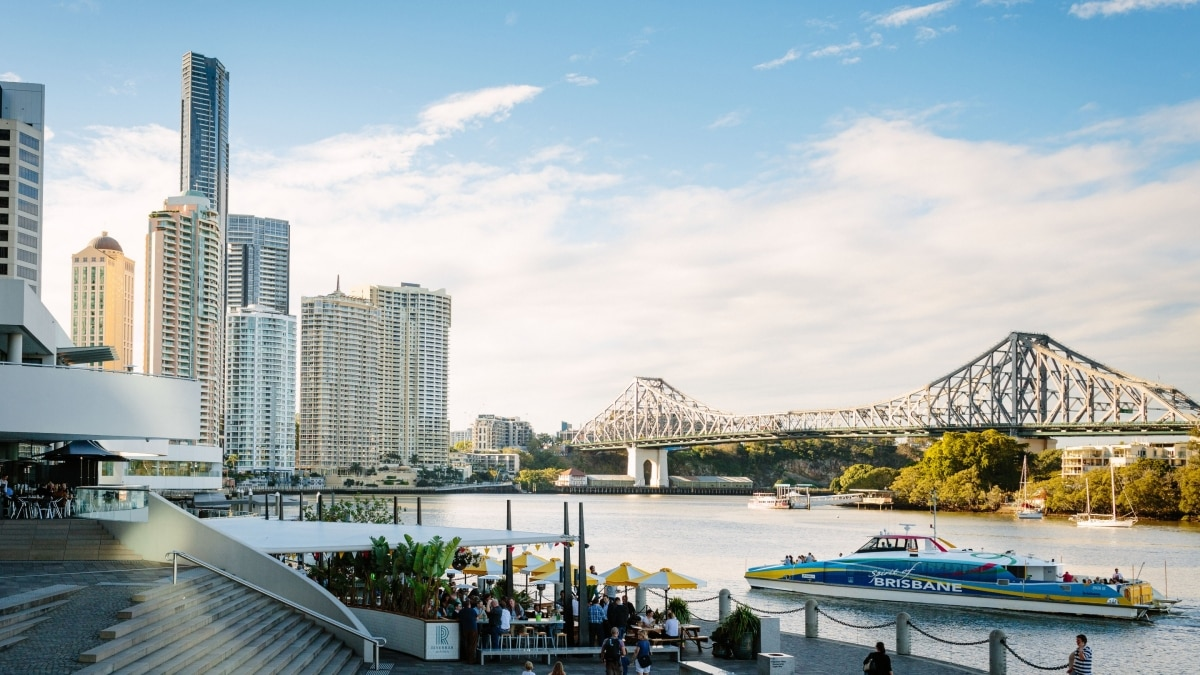
\includegraphics[width=0.9\textwidth]{image/brisbane.jpg}
\end{center}
\end{frame}

\begin{frame}
\frametitle{Queensland}
\begin{center}
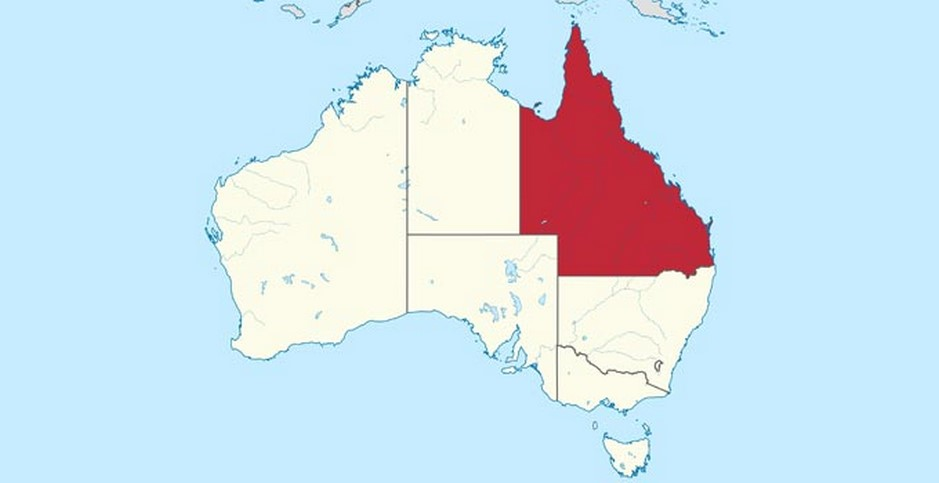
\includegraphics[width=0.9\textwidth]{image/queensland.jpg}
\end{center}
\end{frame}

\begin{frame}
\frametitle{Brisbane east coast}
\begin{center}
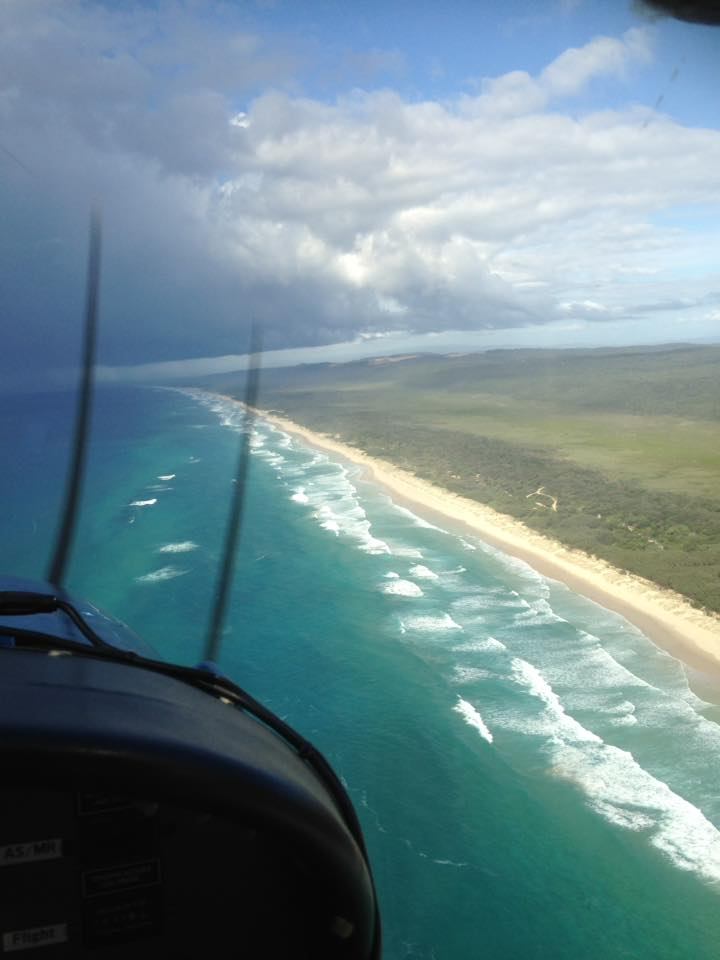
\includegraphics[width=0.5\textwidth]{image/20180420-vh-afr_00.jpg}
\end{center}
\end{frame}

\begin{frame}
\frametitle{QFPL \lstinline{<http://qfpl.io/>}}
\begin{center}
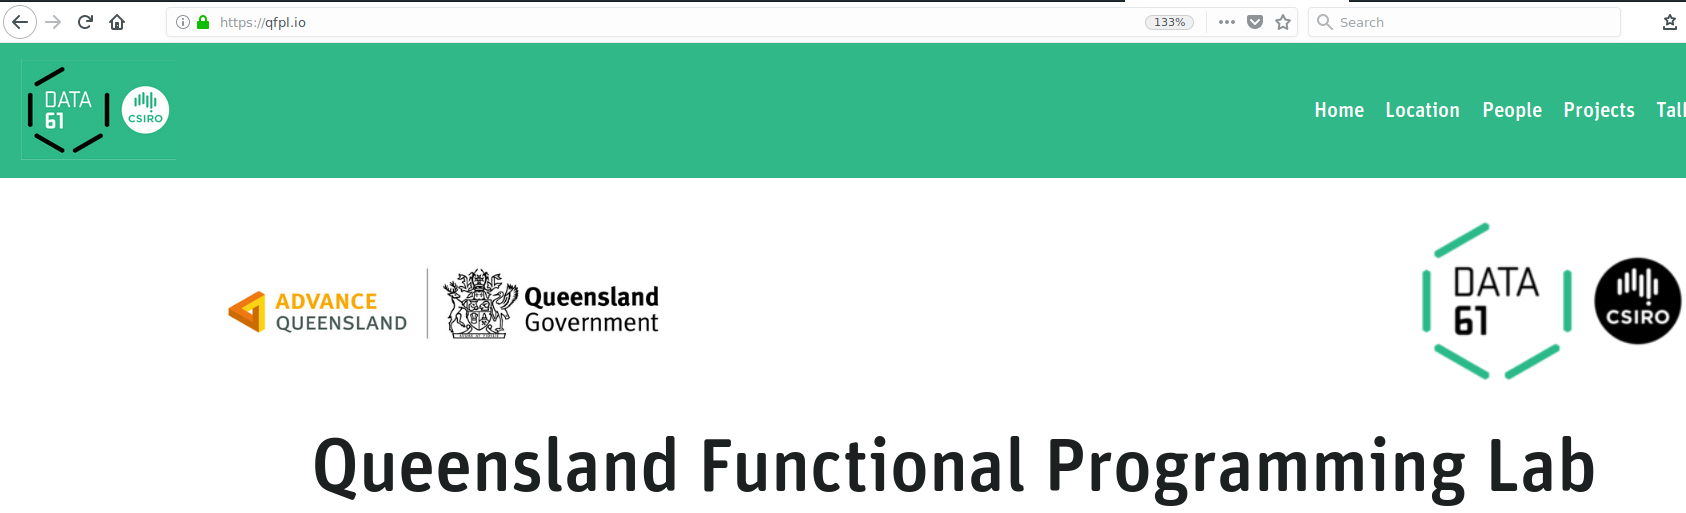
\includegraphics[width=0.9\textwidth]{image/qfpl_io.png}
\end{center}
\end{frame}

\begin{frame}
\frametitle{FAQ}
\begin{quote}
I have heard of these folds \ldots left and right
\begin{itemize}
\item What do they do?
\item How do I know when to use them?
\item Which one do I use?
\item Can I \emph{internalise} how they work?
\end{itemize}
\end{quote}
\end{frame}
